% !TEX root = ../Diplombericht.tex
\newpage
\section{Realisierung} 
\label{sec:Realisierung}
Dieses Kapitel beschreibt, in welcher Reihenfolge der Cluster aufgebaut wurde. Einen tieferen Einblick des Aufbaus und der verwendeten Installationsbefehle kann dem Anhang B entnommen werden. Die Anleitungen zu den Vorbereitungen der Installation sind im Anhang A vermerkt. Weiterhin ist das Betriebshandbuch mit den gängigsten Aufgaben und Befehlen für die Verwaltung des Clusters im Anhang C zu finden.
% !TEX root = ../Diplombericht.tex
\subsection{Physischer Aufbau}

\subsubsection{Komponenten Platzierung}
Der Cluster ist in einem Gestell, welches 4 Ebenen hat, implementiert. Die Ebenen sind wie folgt aufgeteilt: \newline

\begin{figure}[htb]
\centering
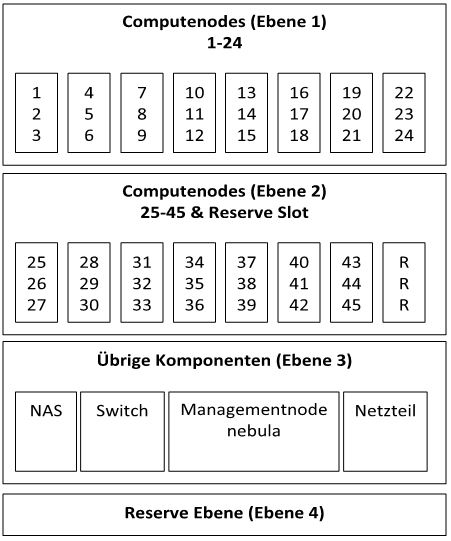
\includegraphics[scale=0.5]{Cluster_Aufbau_Gestell.jpg}
\caption{Physischer Aufbau}
\label{fig:Physischer Aufbau}
\end{figure} 

\textbf{Ebene 1}\newline
24 RPI's sind auf dieser Ebene befestigt worden.

\textbf{Ebene 2}\newline
Es befinden sich 21 RPI's auf dieser Ebene. Es können noch 3 weitere platziert werden.

\textbf{Ebene 3}\newline
Hier wurden alle übrigen Komponenten befestigt. Darunter ist das NAS, der Switch, der Management Node und das Netzteil zu finden.

\textbf{Ebene 4}\newline
Auf dieser Ebene wurde nichts installiert. Sie kann als Reserve Ebene betrachtet werden.

\subsubsection{Kühlung}
Die CPU, RAM und GPU der RPI's wurden mit Aluminium-Kühlkörpern ausgestattet. Die passive Kühlung soll die übertakten CPU's der RPI's am laufen halten.

\subsubsection{Stromversorgung}
\textbf{Compute Nodes}\newline
Die Compute Nodes wurden über die GPIO Pins 2 (5 Volt Anschluss) und 6 (Ground (GND) Anschluss) über Jumperkabel und weiteren Leiterkabeln, welche zur Verlängerung dienen, mit dem Netzteil verbunden. Es wurde darauf geachtet, dass der Kabeldurchschnitt für eine Anzahl von mindestens 25 Ampere ausreicht, so dass diese nicht durchbrennen.

\textbf{Netzteil}\newline
Am Netzteil wurden Kabelschuhe befestigt, welche es ermöglichen, eine Verbindung mit den Leitern in Richtung RPI's herzustellen. Das Netzteil ist an einer gewöhnlichen Stromschiene angeschlossen.

\textbf{Generelle Verkabelung}\newline
Die Leiter wurden hauptsächlich mit Lüsterklemmen verlängert und auf das zusammenlöten der Komponenten wurde deswegen verzichtet. Dies bietet für neue Verkabelungen eine grössere Flexibilität.

\subsubsection{Kommunikation}
Alle Komponenten, welche eine Netzwekverbindung benötigen, sind über den Switch mit Patchkabeln zusammengeschlossen worden. Es wurde dabei keine spezielle Slotzuweisung des Switches berücksichtigt.



% !TEX root = ../Diplombericht.tex
\subsection{Technischer Aufbau}
\subsubsection{Betriebssystem}
Es exisitiert zur Zeit kein 64-Bit CentOS Kernel, welcher mit den RPI's kompatibel ist. Deswegen wurde mit einer alternativen Lösung das Gentoo Image vom Github Repository\footnote{\url{https://github.com/sakaki-/gentoo-on-rpi3-64bit}} von Sakaki heruntergeladen und auf die SD-Karte geschrieben. Dabei wurden zwei Partitionen erstellt: Die Boot-Partition, welche den Kernel und die Bootbefehle beinhaltet, und die Dateisystem-Partition. Diese beinhaltet die Ordnerstruktur und Dateien des Betriebssystems. Diese Partition muss mit der eines CentOS Dateisystems überschrieben werden. Dabei wurde das Dateisystem aus dem offiziellen Repository von CentOS\footnote{\url{http://mirror.centos.org/altarch/7/isos/aarch64/CentOS-7-aarch64-rootfs-7.4.1708.tar.xz}} heruntergeladen und auf die Dateisystem Partition kopiert.

\subsubsection{Vorbereitungen}
\textbf{Netzwerk}\newline
Die IP- und Hostnamenzuweisung wurde über die Internetbox von Swisscom eingerichtet. Dabei wurden alle RPI's an das Netzwerk und den Strom angeschlossen. Nach ca. 2 Minuten wurden alle angeschlossenen Geräte im Interface aufgelistet und konnten anhand des Hostnamenkonzeptes eingerichtet werden.

\textbf{Netzwerkboot}\newline
Der Management Node dient als Provider und verteilt das Betriebssystem an alle angeschlossenen Compute Nodes. Diese mussten vorgängig bearbeitet werden und benötigen bei einem Power On einen One Time Programmable (OTP) Eintrag. Dadurch wird eine Anfrage von jedem Compute Node (Client) an den Management Node gestellt, ob es das Betriebssystem erhalten darf. Zeitgleich wurden noch alle MAC-Adressen ausgelesen, diese werden später für die statische Zuweisung von IP Adressen und Hostnamen benötigt.

\subsubsection{Installation}

Während der Realisierung wurde nach Erfolgserlebnissen jeweils ein aktueller Snapshot der SD-Karte mit dem Programm Win32DiskImager erstellt. Dadurch war es möglich, ein rasches Vorantreiben der Installation zu gewährleisten. Falls zuviele Änderungen am System vorgenommen wurden, welche nicht mehr rasch rückgängig gemacht werden konnten und Probleme verursachten, wurde als Wiederherstellung eines funktionierenden Systems der letzte Snapshot wieder eingespielt.

Zudem wurde für die Installation des Clusters und dessen Komponenten die Installationsanleitung (Install guide with Warewulf + Slurm) von OpenHPC verwendet. Dabei wurde der Warewulf Part zu einem grossen Teil übersprungen. Dieser hätte es ermöglicht, einen vereinfachten Netzwerkboot der Compute Nodes einzurichten. Es ist aber leider nicht möglich, die RPI's damit zu managen, da Warewulf iPXE benutzt und dies nicht kompatibel mit den RPI's ist.










